
%(BEGIN_QUESTION)
% Copyright 2010, Tony R. Kuphaldt, released under the Creative Commons Attribution License (v 1.0)
% This means you may do almost anything with this work of mine, so long as you give me proper credit

Calculate the weight supposing the applied air pressure is just enough to lift it against gravity.  Assume a piston with an outside diameter of 15.2 inches and a rod diameter of 2.8 inches:

$$\includegraphics[width=15.5cm]{i04350x01.eps}$$

Weight = \underbar{\hskip 50pt} lbs

\vskip 10pt

Also, identify whether the solenoid valve needs to be {\it energized} or {\it de-energized} in order to lift the weight.

\underbar{file i04350}
%(END_QUESTION)





%(BEGIN_ANSWER)

I recommend assigning 7 points for the correct weight answer, and 3 points for the correct solenoid answer:

\vskip 10pt

Weight = \underbar{\bf 28,800 lbs}

\vskip 10pt

The solenoid needs to be {\bf energized} in order for the cylinder to lift the weight.

%(END_ANSWER)





%(BEGIN_NOTES)

{\bf This question is intended for exams only and not worksheets!}.

%(END_NOTES)


